\section{Introduction to analytic information theory}

\emph{Data compression}, \emph{source coding}, or 
\emph{bit-rate reduction} involves encoding 
information using fewer bits than its original
representation.
In order to study it we formally define what is 
a data compression scheme. 
First, we describe an algorithm which operates on words - 
in our case, Lempel-Ziv'78.
Then, we introduce a probabilistic model representing
the data to be compressed, which allows us to quantify
the efficiency of the algorithm.


\subsection{Compression scheme: Lempel-Ziv'78 }

\begin{definition}
    A \emph{\bfseries compression scheme} is a pair of functions on
    words $(\mathcal{C}, \mathcal{D})$ \textit{i.e.} a compression 
    and decompression algorithm.
\end{definition}

\begin{definition}
    \label{def:lossless}
    A \emph{\bfseries lossless} compression algorithm decompresses 
    the exact same data that was compressed in the first place.
\end{definition}

% \begin{rmk}
%     We will not describe the decompression part of 
%     our algorithms, considering that the possibility
%     of decompression is obvious in the case of LZ78.
% \end{rmk}

\noindent
In general, Lempel-Ziv algorithms are dictionary-based scheme
which exploit previously seen patterns and redundancy to 
save coding space. 
The Lempel-Ziv'78 (LZ'78) partitions a sequence into 
\emph{phrases} or \emph{blocks} of variable size such that a new phrase
is the shortest substring not seen in the past as a phrase. 
Every such phrase is encoded by the index of its prefix 
appended by a symbol; thus the LZ'78 code contains the 
pairs \verb|(pointer, symbol)|. 
For example, the string 
\centers{$w = 11001010001000100$}
\noindent of length 17 is parsed
as 
\centers{()(1)(10)(0)(101)(00)(01)(000)(100)}
\noindent
which can be be 
encoded in the following associated \emph{digital search tree} (DST) $\mathcal{T}(w)$:

\centers{
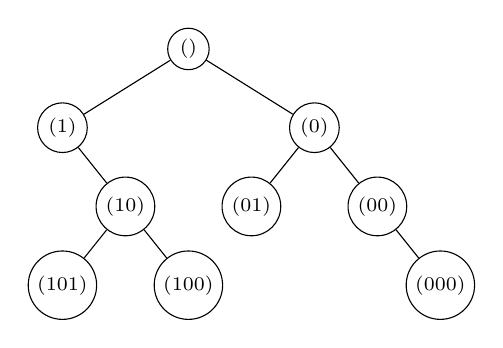
\begin{tikzpicture}[
    level 1/.style={level distance=10mm,sibling distance=32mm},
    level 2/.style={level distance=10mm,sibling distance=16mm},
    level 3/.style={level distance=10mm,sibling distance=16mm},
    font=\scriptsize,inner sep=2pt,every node/.style={draw,circle,minimum size=3ex}]
  ]
  \node {()}
    child {node {(1)}
        child[missing]
        child {node {(10)}
            child {node {(101)}}
            child {node {(100)}}
        }
    }
    child {node {(0)}
        child {node {(01)}}
        child {node {(00)}
            child[missing]
            child {node {(000)}}
        }
    }
        ;
\end{tikzpicture}
}

\begin{rmk}
    \label{rmk:dst}
    Given a digital search tree $\mathcal{T}(w)$
    (DST) and the order of arrival of its nodes, we can 
    reconstruct the original sequence $w$.
\end{rmk}

\begin{rmk}
    See Appendix~\ref{app:lempelziv} 
    for a pseudocode of the encoding part of LZ'78.
\end{rmk}


\subsection{Probabilistic models }

\begin{df}
    \label{def:source}
    Let $\mathcal{A}$ be an alphabet.
    An \emph{\bfseries information source} is a one-sided infinite sequence of random
    variables $(X_k)_{k=1}^{\pinf}$ with each $X_k$ being one
    symbol random variable with values in $\mathcal{A}$.
\end{df}

\begin{rmk}
    \label{rmk:sequence}
    Each finite section of the realization of an information source is called a 
    \emph{\bfseries sequence} or \emph{\bfseries word}. For example: $X_m \dots X_{m+n-1}$
    realizes into words of size $n$.
\end{rmk}

\begin{rmk}
    \label{rmk:source}
    Defining the law of the $X_k$ produces out different
    models for data generation which can be studied mathematically
    and simulated.
\end{rmk}

\begin{df}
    \label{def:memoryless}
    A \emph{\bfseries memoryless source} is an \emph{information source}
    for which the $X_k$ are independent, following
    the uniform law on $\mathcal{A} = \{ a_1, \dots, a_V \}$ :
    \centers{$
        \proba{  X_k = a_k  } = p_k 
        \qquad \textmd{with } \,\Sum{i=1}{V} \,p_i = 1
    $}
\end{df}

\begin{rmk}
    \label{rmk:memoryless}
    This is the simplest information source and it has been 
    studied successfully in the past, but it is not a realistic 
    model. We replace it with the following Markov source model whenever 
    possible.
\end{rmk}

\begin{df}
    \label{def:markov}
    A \emph{\bfseries Markov source} is an \emph{information source}
    with a Markov dependency between successive symbols.
\end{df}

\begin{df}
    \label{def:markovorder}
    A \emph{\bfseries Markov source of order $r$} is a Markov source
    for which each symbol apparition depends on the previous 
    $r$ symbols.
\end{df}

\begin{rmk}
    \label{rmk:markov2}
    We will study Markov sources of order 1, where each
    symbol simply depends on the previous one. This is 
    general enough, as Markov sources of superior order
    can be simulated with a Markov source of order 1 
    while expanding the alphabet.
\end{rmk}

\subsection{Entropy}

    For a consistent set of notions surrounding information theory,
    I consulted chapter 6 of~\cite{szpankowski_average_nodate}.
    In this study, we will only consider two information sources:
    the \emph{\bfseries memoryless} and the \emph{\bfseries Markov} source.
    There are other types of probabilistic information sources 
    described in~\cite{jacquet_analytic_2015} which I found interesting,
    but had no occasion to use them in practice.
    For the Markov source, we consider that there exists a 
    \emph{\bfseries stationary distribution} $\pi = (\pi_1,\dots,\pi_V)$.
    

    \begin{df}
        \label{def:entropy}
        The \emph{\bfseries entropy} of an information is the average
        rate at which information is produced by a probabilistic
        source of information.
    \end{df}

    \begin{prop}
        \label{prop:memorylessentropy}
        The entropy of a \emph{memoryless source} on 
        alphabet $\mathcal{A} = \{ a_1,\dots,a_V \}$ is
        \centers{$ h = -\Sum{i=1}{} p_i \log p_i$}
    \end{prop}

    \begin{prop}
        \label{prop:markoventropy}
        The entropy of a \emph{Markov source} with probability
        $(p_{i j})_{(i, j) \in { \{1,\dots,V\} }^2} $ and a 
        stationary distribution $(\pi_1, \dots, \pi_V)$ is
        \centers{$ h = -\Sum{i=1}{} \pi_i \Sum{j=1}{} p_{i j} \log p_{i j} $}
    \end{prop}

    
\subsection{Probabilistic analysis }

Under this context, we can define and conduct a thorough
analysis of several random variables with different meanings
regarding the effectiveness of compression.

\begin{nota}
    \label{nota:universe}
    Let $n$ be an integer - the size of the considered words.
    Defining $\Omega_n$ the \emph{\bfseries set of words of size $n$} on alphabet
    $\mathcal{A}$. Each word being an event, a natural probability
    space is given by considering the output of size $n$ of a Markov
    source.
\end{nota}

\begin{rmk}
    \label{rmk:probaspace}
    We will now study random variables defined 
    on this probability space. 
\end{rmk}

\begin{nota}
    \label{nota:output}
    The random variable $W_n$ denotes words of size $n$ output by a given Markov source.
\end{nota}

\begin{nota}
    \label{nota:numberphrases}
    The number of phrases used to compress words of size $n$ ($W_n$) with
    LZ'78 is given by $M_n(W_n)$ or simply $M_n$.
\end{nota}

\begin{rmk}
    \label{rmk:numberphrases}
    This is one of the most important variables to consider because,
    as it will appear shortly, it is closely tied to the \emph{compression 
    ratio} of LZ'78.
\end{rmk}

\begin{df}
    \label{df:codelength}
    The \emph{\bfseries codelength} is the \emph{\bfseries number of bits} required 
    to encode the LZ'78-compressed version of a word, denoted by $|C(W_n)|$ or 
    simply $C_n$.
\end{df}

\begin{df}
    \label{df:compratio}
    The \emph{\bfseries compression ratio} for words of size $n$ is the ratio between the 
    codelength and the size of a word
        \centers{$\rho_n = \f{C_n}{n}$}
\end{df}

\begin{prop}
    The compression code $C(w)$ is a description of the DST $\mathcal{T}(w)$,
    node by node in the order of creation. Each node being identified by a node 
    to its parent node in the tree and the symbol that labels the edge linking it to the
    parent node. The pointer to the $k$th node requires at most $\ceil{\log_2(k)}$ bits,
    and the next symbol costs $\ceil{\log_2 |\mathcal{A}|}$ bits. Therefore, the 
    compressed code length is 
    \centers{$|C(w)| = \Sum{k=1}{M_n(w)} \pa{\ceil{\log_2(k)} + \ceil{\log_2 |\mathcal{A}|}}$}
\end{prop}




    \noindent
    We focus now, as stated in the title of this report, on the asymptotical behavior,
    for $n \rightarrow \pinf$, of the compression ratio. Certainly this gives us 
    information about real-world compression, as files on our computer often attain
    large numbers when measured in bits. However, this assumption can be nuanced.
    For example, the speed of convergence towards this asymptotic behavior can make 
    a non-negligible difference in real-world application, as we will see later on
    when we talk about the difference between LZ'77 and LZ'78 and Optimal Parsing.


\subsection{Theorems and Goals }

    There is a number of interrogations and results that surround
    the LZ'78 compression scheme, and that have been doing so for 
    some time now. These were proven for the simpler memoryless
    source model in~\cite{louchard_average_1995} 
    and~\cite{jacquet_limiting_2014}, and
    will allow us to formulate these as 
    theorems for memoryless sources. But the more difficult case
    of Markov sources has all these theorems become conjectures.
    My first job was to simulate the compression scheme and output visualizations
    that would disprove or make these results seem likely.

    

    \begin{prop}
        \label{prop:lowerbound}
        The entropy gives a lower bound on the compression 
    ratio of lossless algorithms. For a memoryless or Markov source, the average compression ratio
    tends asymptotically to the entropy of the source:
        \centers{$\underset{n\rightarrow\pinf}{\limt}\f{E[C_n]}{n} = h$}
    \end{prop}

    \begin{theo}
        The random variable $M_n$ over the LZ'78 compression of a sequence 
        generated by a memoryless source asymptotically obeys a
        \emph{\bfseries central limit law} in the
        sense that its distribution is \emph{\bfseries asymptotically normal}.
        That is, for all $x = \grando(1)$,
        
          \centers{$ \underset{n\rightarrow\pinf}{\limt}
          \proba{\f{M_n-E[M_n]}{\sqrt{\Var[M_n]}} \leq x}
              = \f{1}{\sqrt{2\pi}} \Int{\minf}{x} 
                                      \ex{-\tf{t^2}{2}}\dt$}
    \end{theo}

    \begin{rmk}
        \label{rmk:clt}
        This is the result that we will refer to as CLT 
        for LZ'78 on Markov sources. It has remained an open
        for around twenty years, as it was proved for 
        memoryless sources in~\cite{jacquet_average_2001}.
    \end{rmk}

    % \begin{th}
    %     \label{th:clt}
    %     For memoryless source
    % \end{th}
